\chapter{Implementation}

In this chapter a way to implement a system like the one described in Chapter 3 will be explained by an example based on TinyOS.    

\section{General Structure}
The system is dividable into two main components. The base station, that stores and processes the data, and the motes, that collect the data. Both parts of the system need their own hard- and software to complete their tasks.  
\subsection{General Base Station}

\begin{figure}[htbp]
	\centering
    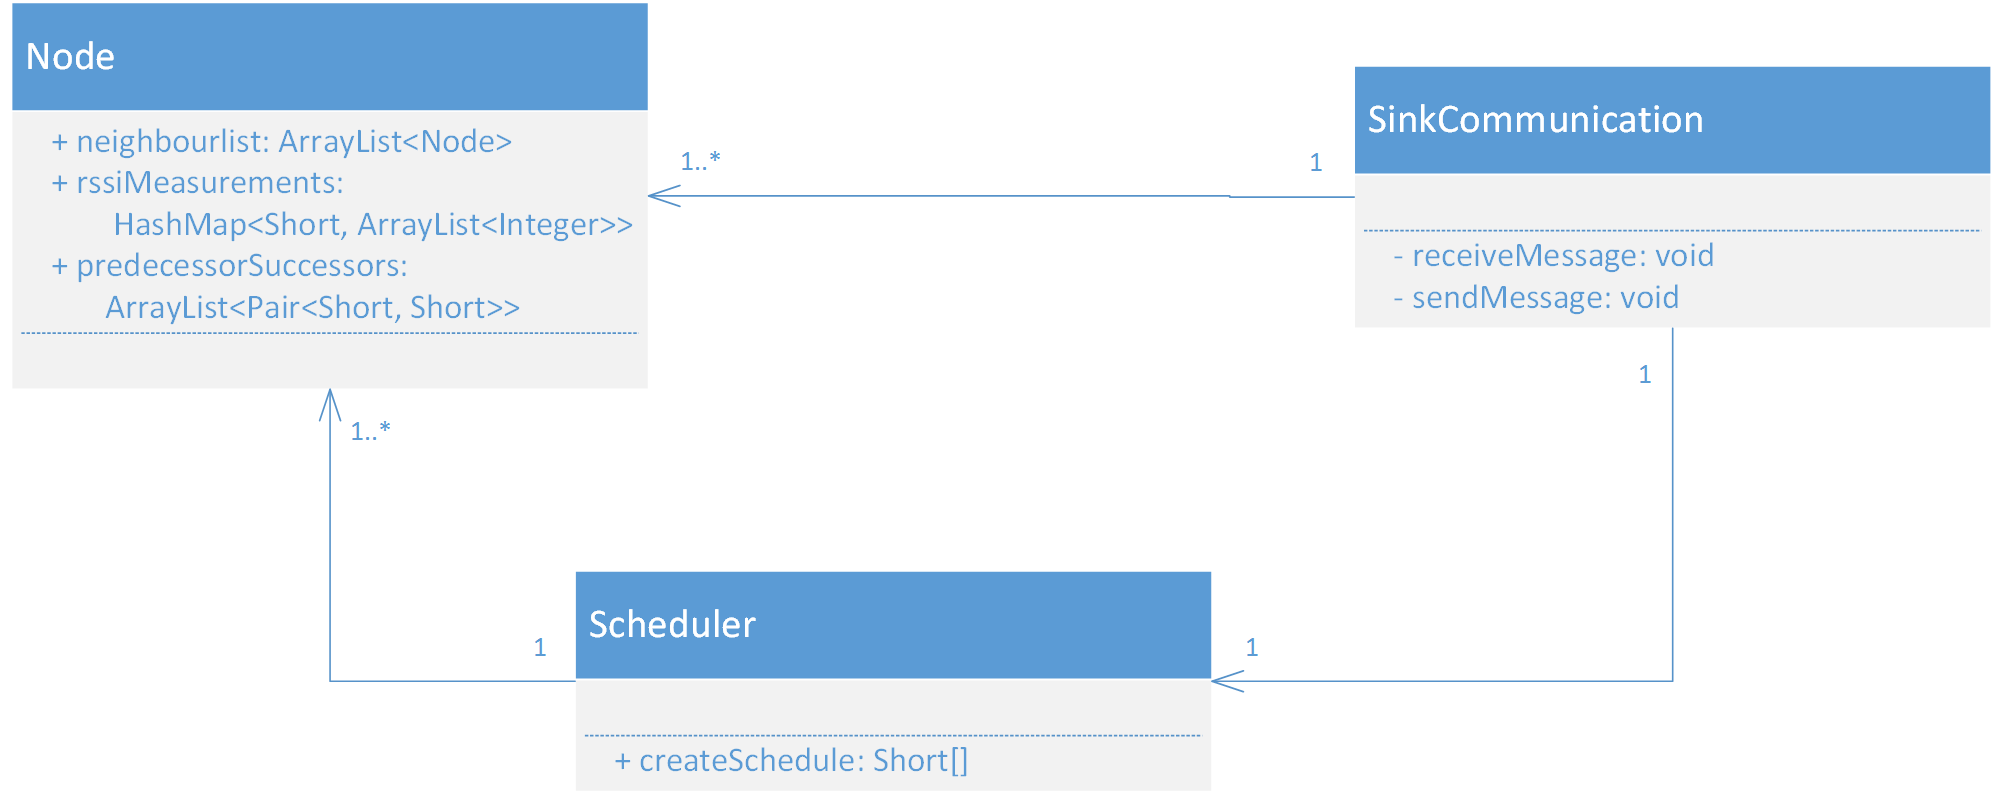
\includegraphics[scale=0.7]{content/images/BaseStation/Klassendiagram}
   	\caption{General structure and functionality of the base station}
    \label{fig:bsKlassen}
\end{figure}

The base station can be a computer running a Java application connected to the sink via a USB-Cable. In Figure \ref{fig:bsKlassen} you can see the general structure of the Java application with its classes and their basic functionality. Firstly there is the SinkCommunication class that handles the communication with the sink. It is responsible for receiving and processing messages and to send messages to the sink. Then there is the Node class which stores all the information about one node. It stores the neighbours of the node, the measurements a node made and its predecessors and successors. The last class is the Scheduler that is responsible of creating a schedule based on the data saved in the node classes.  
\subsection{General Mote Application}
\begin{figure}[htbp]
	\centering
    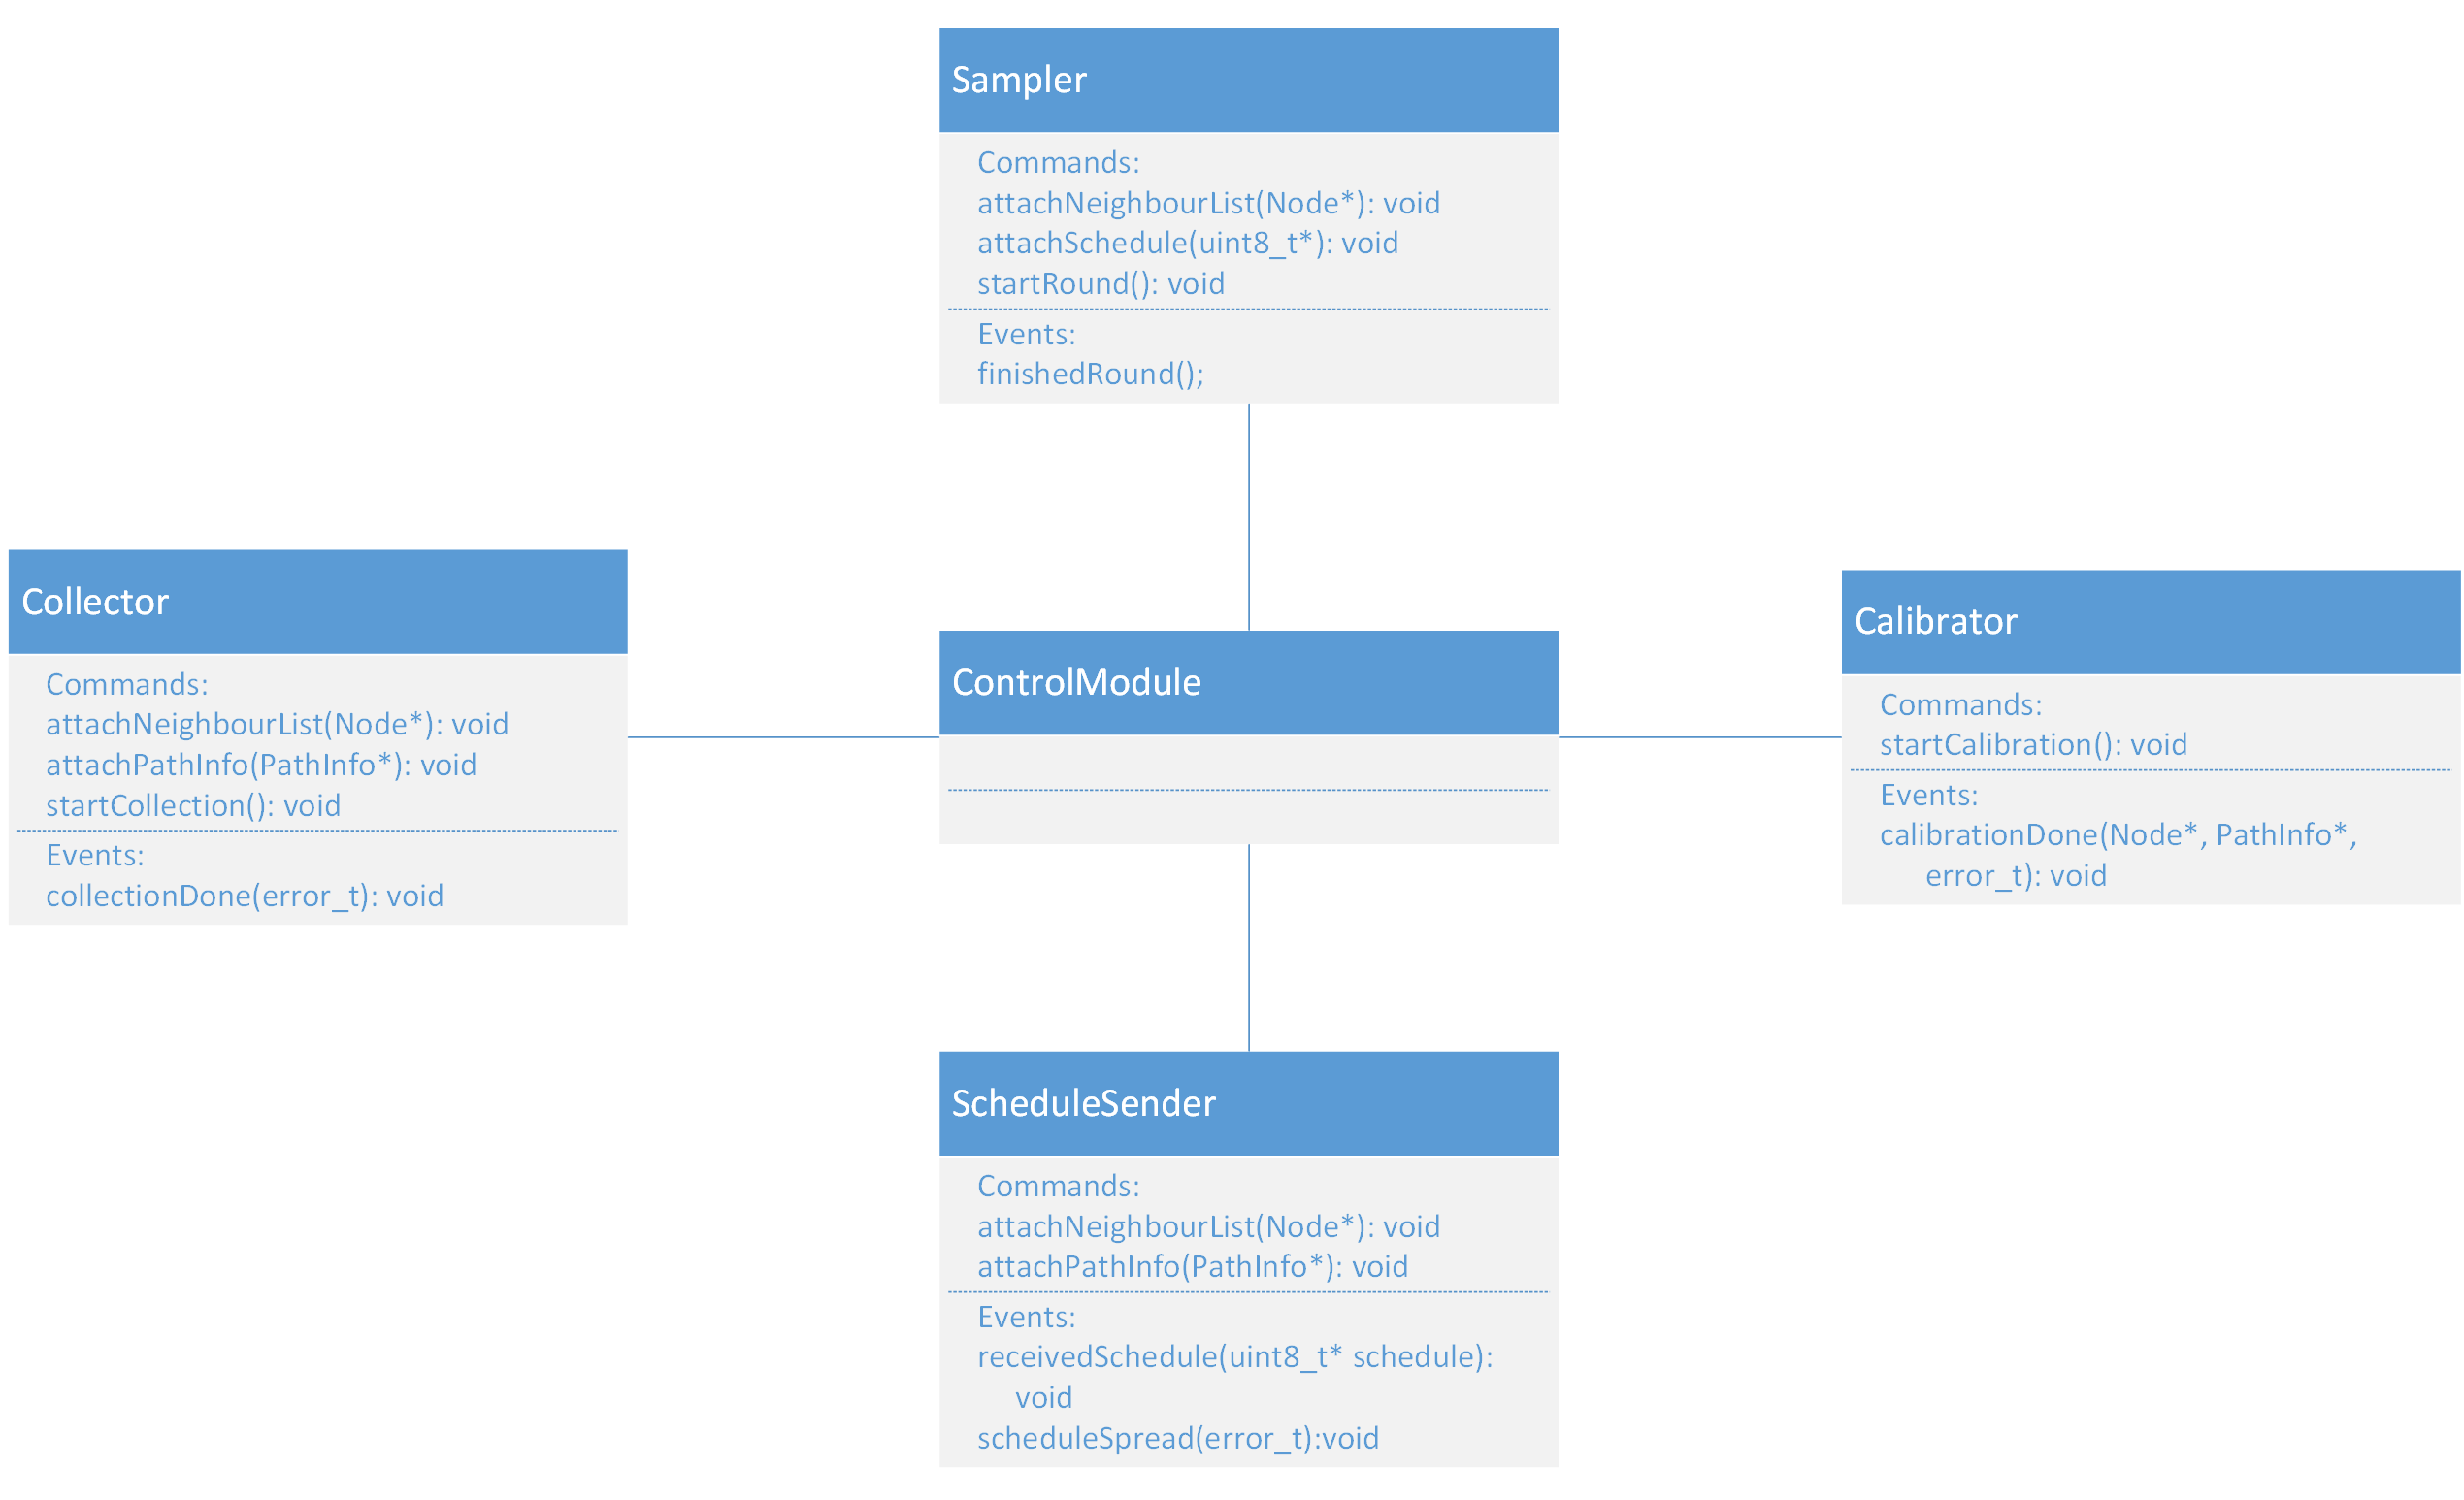
\includegraphics[scale=0.6]{content/images/Motes/GeneralStructure}
   	\caption{The interfaces each module provides. The ControllModule does only use all the other interfaces and does not provide one itself}
    \label{fig:moteStructure}
\end{figure}
The application running on the motes has multiple tasks. It needs to be able to calibrate the network, collect data from the network, spread the schedule inside the network and sample the RSSI. Therefore it can be split into multiple modules with fitting interfaces that each handle exactly one task. The suggested structure of the application is shown in Figure \ref{fig:moteStructure}. The ControllModule connects all the other modules and makes sure the informations the other modules provide get delivered correctly to the modules needing the informations.     

\section{Base Station}
\subsection{Receiving and Storing the Data}

\subsection{Creating the Schedule}
\section{Calibration}
\section{Collection}
\section{Creating the Schedule}
\section{Spreading the Schedule}
\section{Sampling}